\documentclass{article}
\usepackage[fleqn]{amsmath}
\usepackage{graphicx}

% A4 page setup
\topmargin -45pt
\textwidth=532pt
\oddsidemargin=-40pt \evensidemargin\oddsidemargin
\textheight 682pt


\begin{document}
{\centering
\huge
\bf
Homework Assignment 4\\*
\rm
\centering
Rovios and Basic Control\\*
}

\vspace{8mm}

\bf Section 1.1: Obstacle Course Setup \rm

In creating the obstacle course, I was actually rather surprised to see how inconsistently the Rovio robot carried out its orders. Of course, I knew some variation was to be expected, but, the difference in magnitude was enormous. In fact, at times, it seemed as if the motors weren't even being powered consistently, as some of the runs had hiccups. Nevertheless, because of the inconsistency we opted to make the course relatively simple, without it being a straight line.

We ensured good NS visibility by making sure there were as little fixtures on the ceiling as possible in the area we chose, and by making sure the ceiling was relatively flat. As an extra-precaution (knowing that the NorthStar sensor works by reading infrared light), we chose a darker area, as can be seen in the picture below: \\*


{
\centering
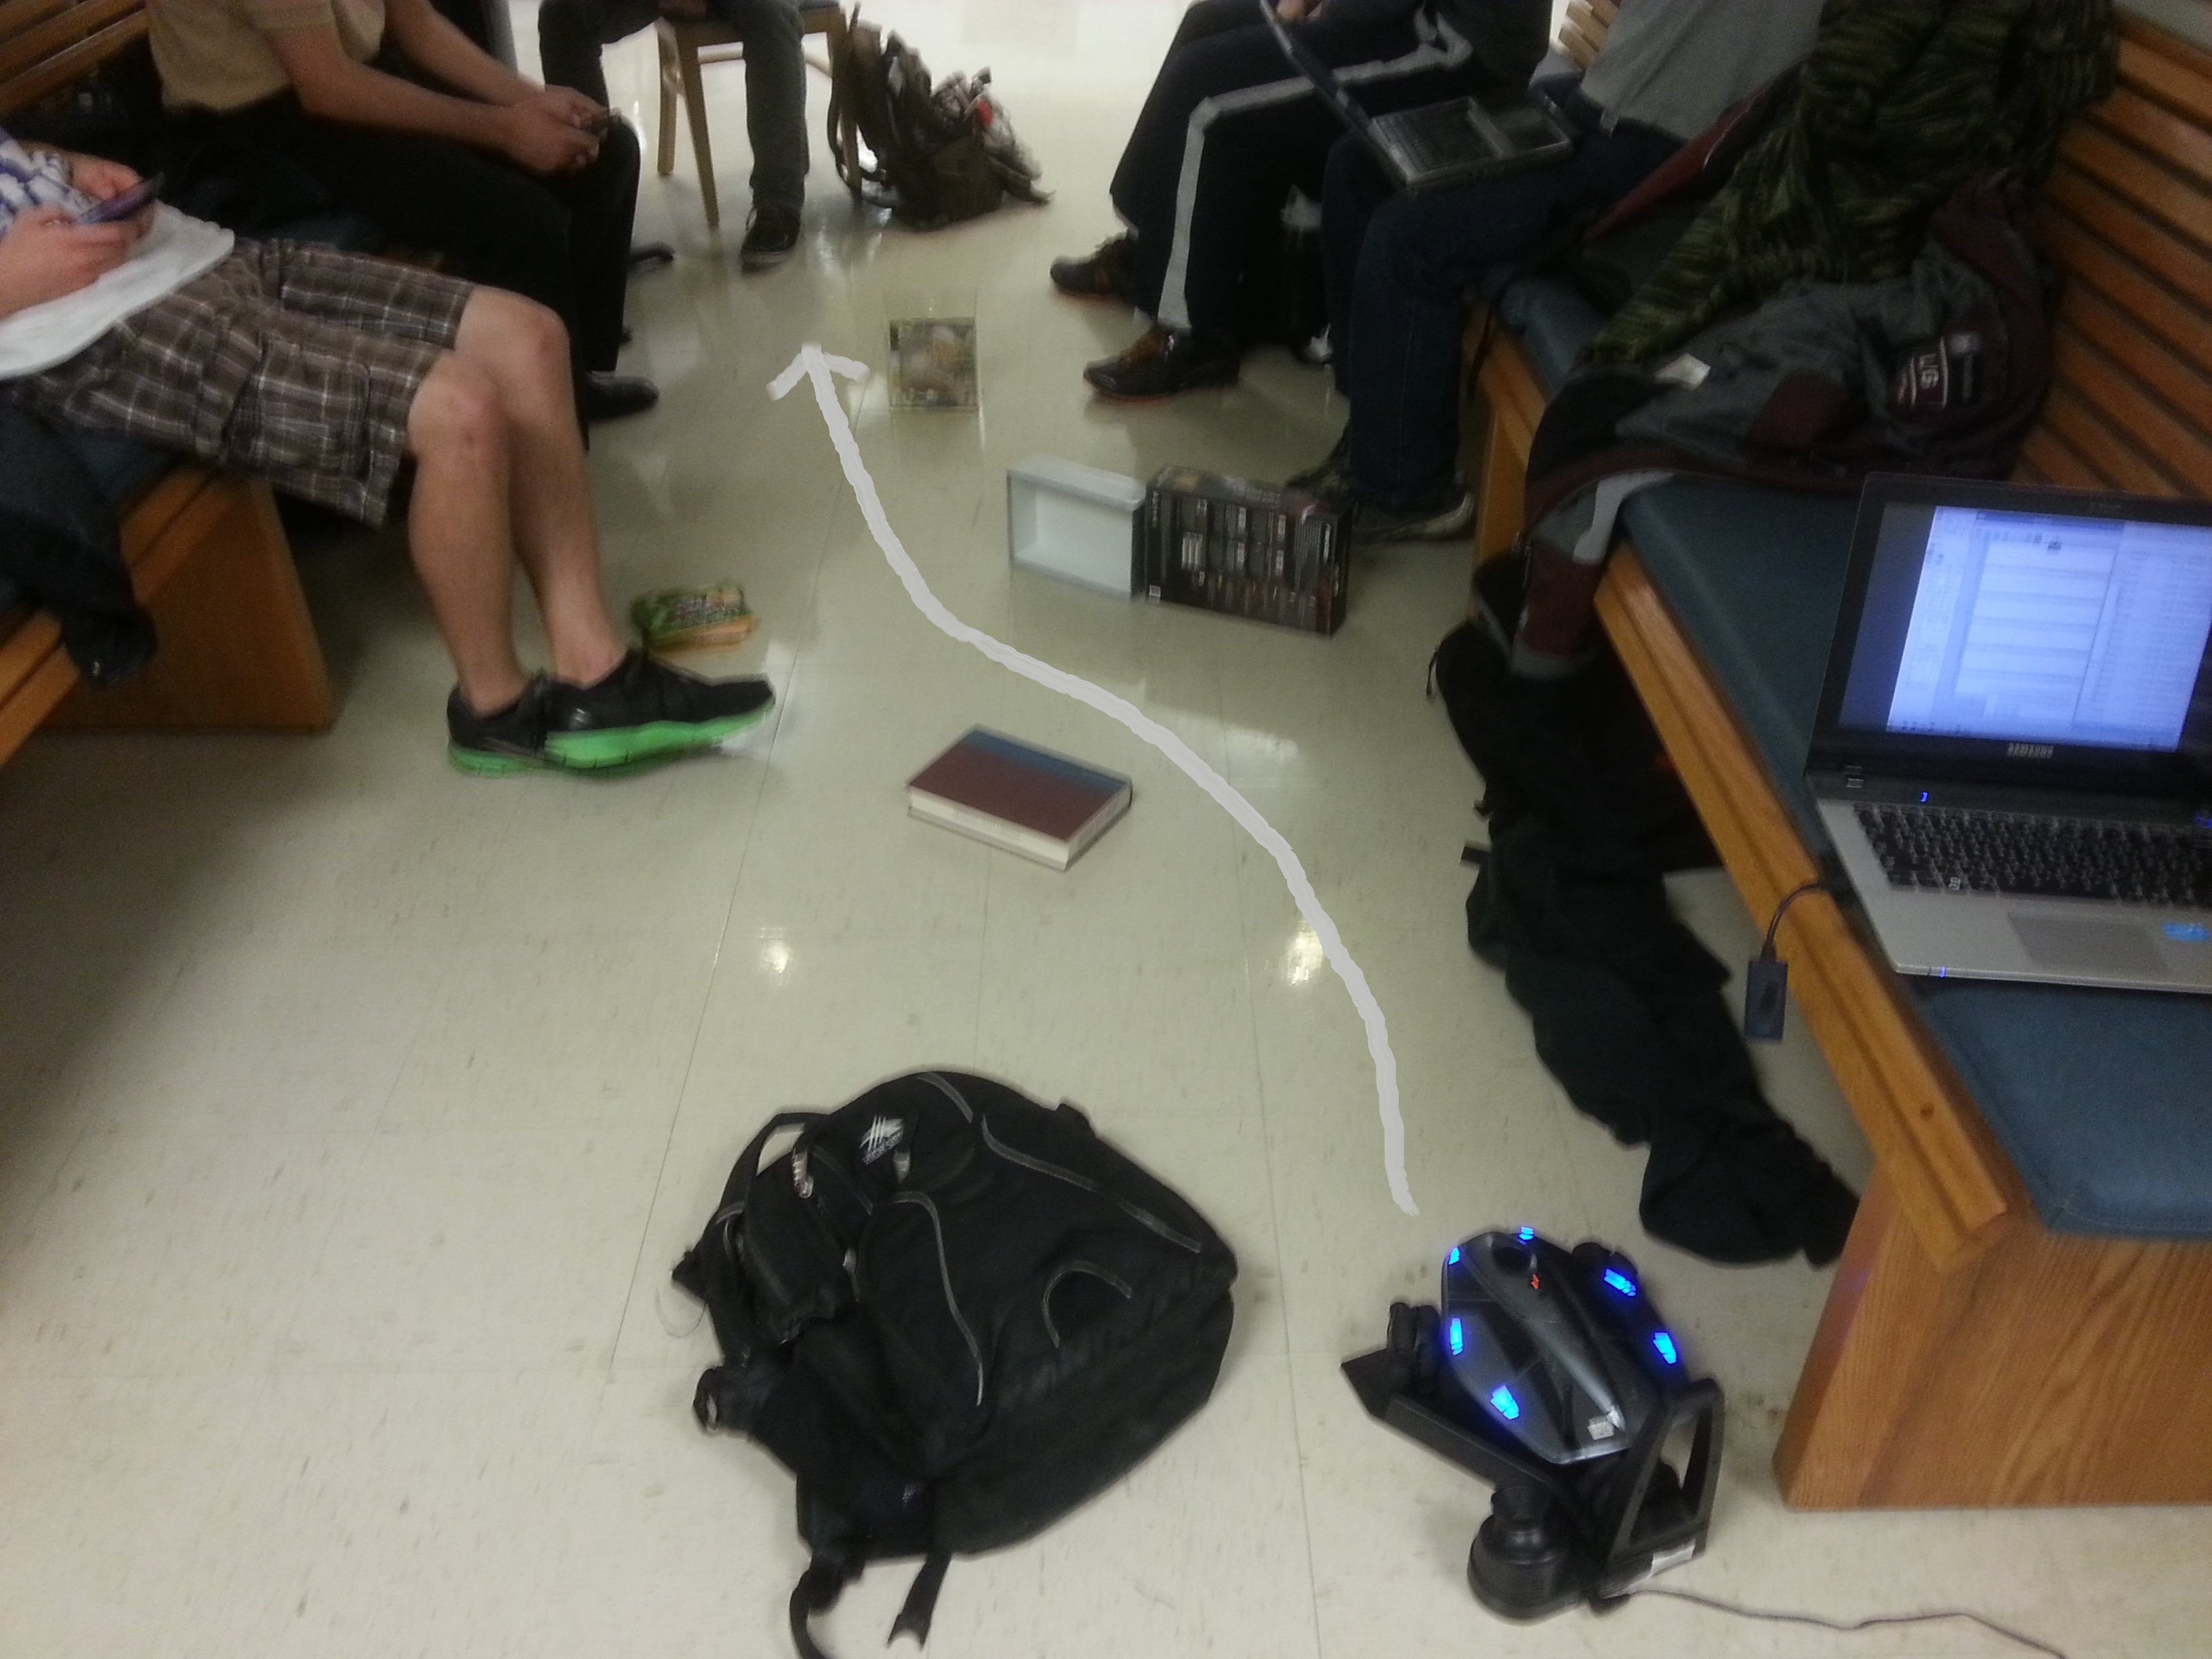
\includegraphics[width=12.5cm]{course.jpg} \\*
}

\vspace{8mm}
\bf Section 1.2: Dead Reckoning Calibration \rm
\vspace{4mm}

Below are the calculated averages for the displacement observed with each of the six commands specified in the homework PDF. These are the calculated means only for all 8 of the samples I took (with a speed of 6 and a duration of 1). For the actual recorded values, you'll want to refer to the included Excel spreadsheet.

\begin{center}
  \begin{tabular}{| l | c | c | r| }
    \hline
    Direction & $\Delta x $ & $\Delta y $ & $\Delta \theta $\\ \hline
    Forward & -12.84 & 13.11 & -0.13 \\ \hline
    Backward & 8.36 & -10.77 & 0.15 \\ \hline
    Right & 10.90 & 9.55 & 0.024 \\ \hline
    Left & -10.42 & -10.86 & -0.085 \\ \hline
    Rotate\_Right & -0.83 & -0.21 & -3.44 \\ \hline
    Rotate\_Left & 0.075 & 0.24 & 2.9 \\
    \hline
  \end{tabular}
\end{center}

\vspace{33mm}
\bf Section 1.3: Odometry Calibration \rm
\vspace{4mm}

As noted in the pdf, the twist of a set of encoder values is:
$$ \dot{\xi} = 
J\left[\begin{array}{c}
\dot{\phi_r} \\
\dot{\phi_l} \\
\dot{\phi_b}
\end{array}\right] \\* 
$$

From this it follows that
$$\left[\begin{array}{c}
\dot{\phi_r} \\
\dot{\phi_l} \\
\dot{\phi_b}
\end{array}\right] = J^{-1}\dot{\xi}
\\* 
$$

For the above equality to be true, we find that $J^{-1}$ must be:
$$
\left[\begin{array}{ccc}
\frac{\partial \phi_r}{\partial x} & \frac{\partial \phi_r}{\partial y} & \frac{\partial \phi_r}{\partial \theta}\\
\frac{\partial \phi_l}{\partial x} & \frac{\partial \phi_l}{\partial y} & \frac{\partial \phi_l}{\partial \theta}\\
\frac{\partial \phi_b}{\partial x} & \frac{\partial \phi_b}{\partial y} & \frac{\partial \phi_b}{\partial \theta}\\
\end{array}\right]
$$

since 
$$ \dot{\xi} = 
\left[\begin{array}{c}
\frac{\partial x}{\partial t} \\
\frac{\partial y}{\partial t} \\
\frac{\partial \theta}{\partial t} 
\end{array}\right] \\* 
$$

and, according to the homework PDF, a reasonable way to approximate these values is to average the values for each of the encoder ticks. Under this configuration, the average ticks for the command ``forwards" end up in the first column, ``left" in the second, and ``rotate\_left" in the third. Using the data included in the Excel file, we get the following approximated inverse Jacobian:

$$J^{-1} =
\left[\begin{array}{ccc}
13.5 & 9.5 & 15.2\\
11.62 & 9.67 & 15.4\\
0 & 20.67 & 15.6\\
\end{array}\right]$$ \\*

Then, we simply invert the matrix to get $J$.

\vspace{4mm}
$$J = (J^{-1})^{-1} =
\left[\begin{array}{ccc}
0.5043 & -0.4999 & 0.0021\\
0.5459 & -0.6342 & 0.0942\\
-0.7233 & 0.8404 & -0.0607\\
\end{array}\right]$$ \\*


\vspace{8mm}
\bf Section 2.1: Expected Trajectory \rm
\vspace{4mm}

forward,6,1\\
rotate\_right,5,0.25\\
forward,6,0.7\\
rotate\_left,5,0.35\\
forward,6,1.9\\
rotate\_right,5,0.25\\
forward,6,1\\

For the given commands, I expected the trajectory to take the following path. I came to this file by adjusting the parameters until I got something that worked most of the time.


\vspace{8mm}
\em But we did this wrong \rm 
\vspace{8mm}
\\*
OK, I must admit, we screwed this up. I didn't realize this until too late, since we had very limited time to meet (we literally had only one 30 minute window all week), and we only read the first part of the assignment while we were meeting. The obstacle course environment and the environment that I took the calibration data in are totally different. So, the data we took doesn't even apply to the obstacle course.

So, upon realizing this, besides becoming very sad, I realized I'd need a way to approximate a transformation between the two coordinate frames. So, using the non-exhaustive data we used in our intial trial runs, I found the displacement vector for the forward command to be 
$$
\vec{v}_{maze} = (10.24, -5.53)^T 
$$

and from the mean values earlier, I can conclude that the displacement vector in the frame that we took data in is
$$
\vec{v}_{test} = (-8.36, 10.77 )^T
$$

so from here, I construct a non- rigid transformation from one north-star frame to the other. Such a transformation $T= RS$ must satisfy the equality $\vec{v}_{maze} = T\vec{v}_{test}$, where $R$ is a rotation matrix and $S = cI$ is a scaling matrix.

After some numerical and analytical analysis, I have concluded that a reasonable transformation is given by:
$$
R = \left[\begin{array}{cc}
0.9149 & -0.4037 \\
0.4037 & 0.9149 \\
\end{array}\right]$$ \\*
$$
S = -0.8536I
$$
so

$$
T = \left[\begin{array}{cc}
-0.7809 & 0.3446 \\
-0.3446 & -0.7809 \\
\end{array}\right]
$$

Nevertheless, for reference, the experimentally-determined ``expected" path is shown below, in black:

{
\centering
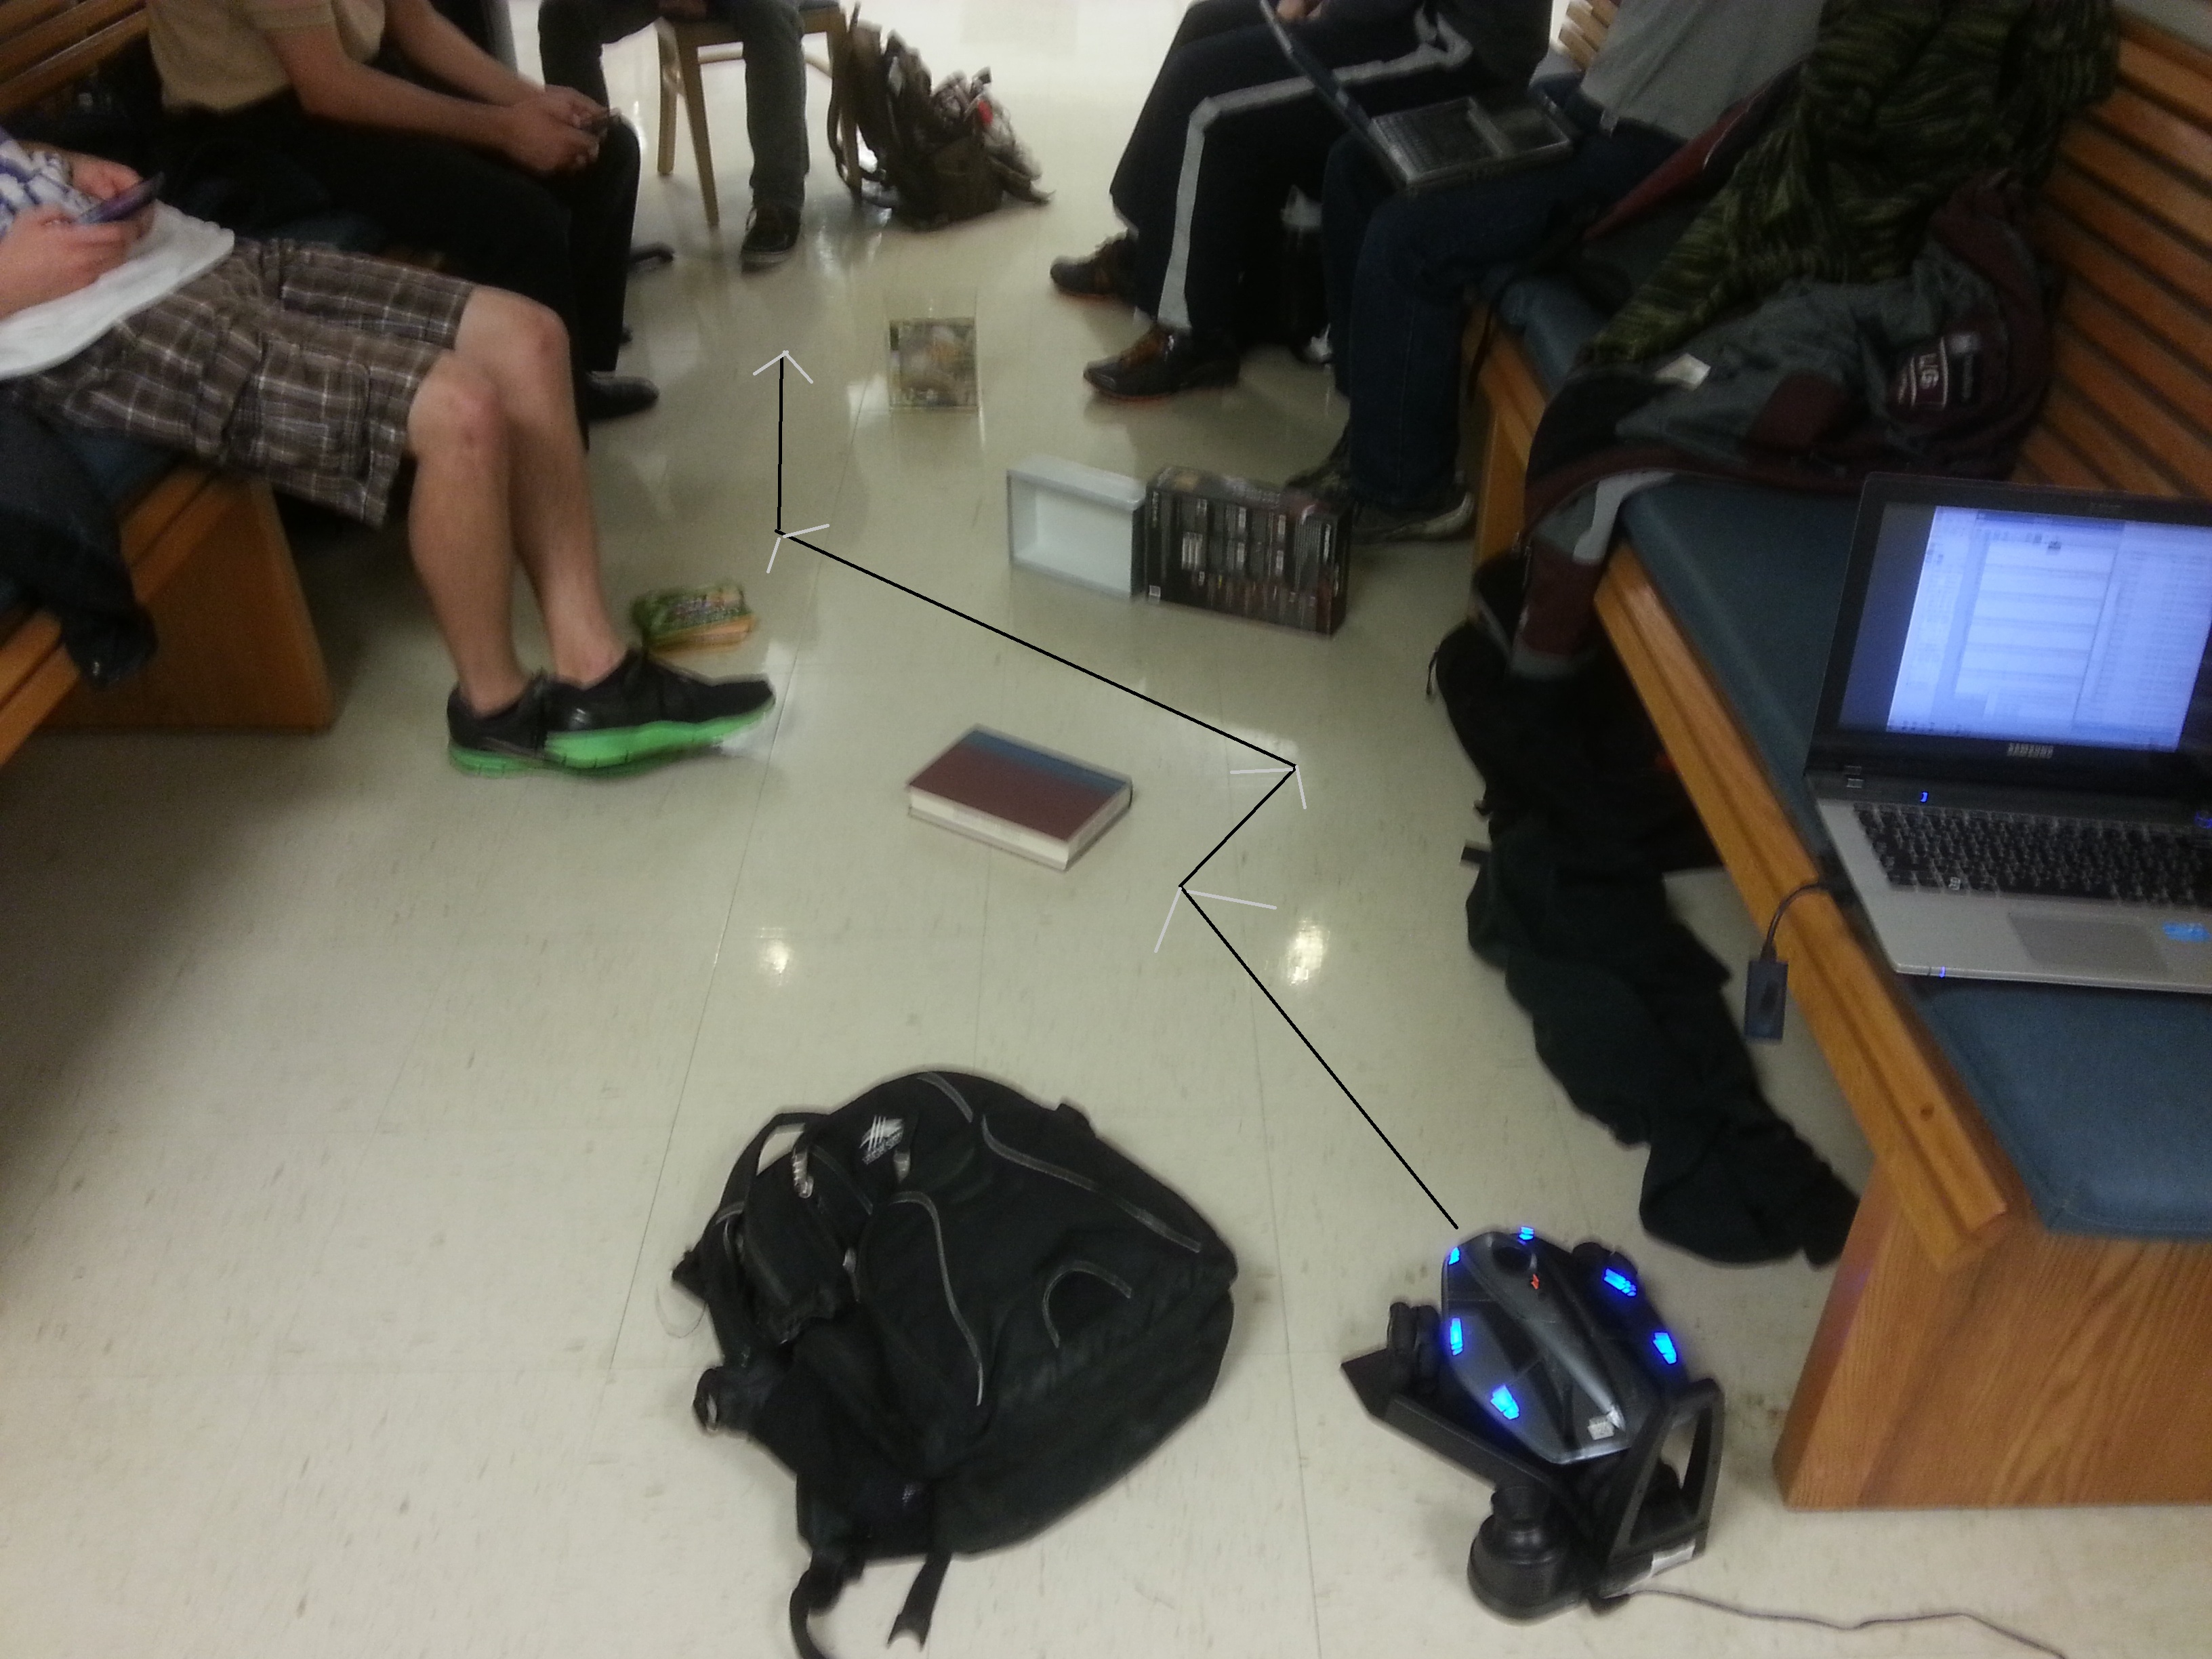
\includegraphics[width=12.5cm]{expected.jpg} \\*
}

\vspace{8mm}
\bf Section 2.2: Trajectory from Dead Reckoning \rm\\
\vspace{4mm}
So now, we can finally get on with this. For each command, I will take the values in the NS frame we took measurements in, and then transform them to the NS frame we had the maze in so I can generate a trajectory.

So first, we do the menial calculations:
$$
\vec{x}^1_{maze} = T(-12.84, 13.11)^T
$$

$$
\vec{x}^1_{maze} = (14.54, -5.81)^T
$$

$$
\vec{x}^2_{maze} = R(\frac{0.25*5}{6}*3.44)(0.7T(-12.84, 13.11)^T)
$$

$$
\vec{x}^2_{maze} = (10.35, 3.62)^T
$$

$$
\vec{x}^3_{maze} = R(\frac{0.35*5}{6}*-2.9 + -0.7167)(1.9T(-12.84, 13.11)^T)
$$

$$
\vec{x}^3_{maze} = (25.98, -14.51)^T
$$

$$
\vec{x}^4_{maze} = R(\frac{0.25*5}{6}*3.44 + 0.1292)(T(-12.84, 13.11)^T)
$$

$$
\vec{x}^4_{maze} = (15.33, 3.22)^T
$$

Then, with these values in mind, I approximately visualized the estimated path in the image below:

{
\centering
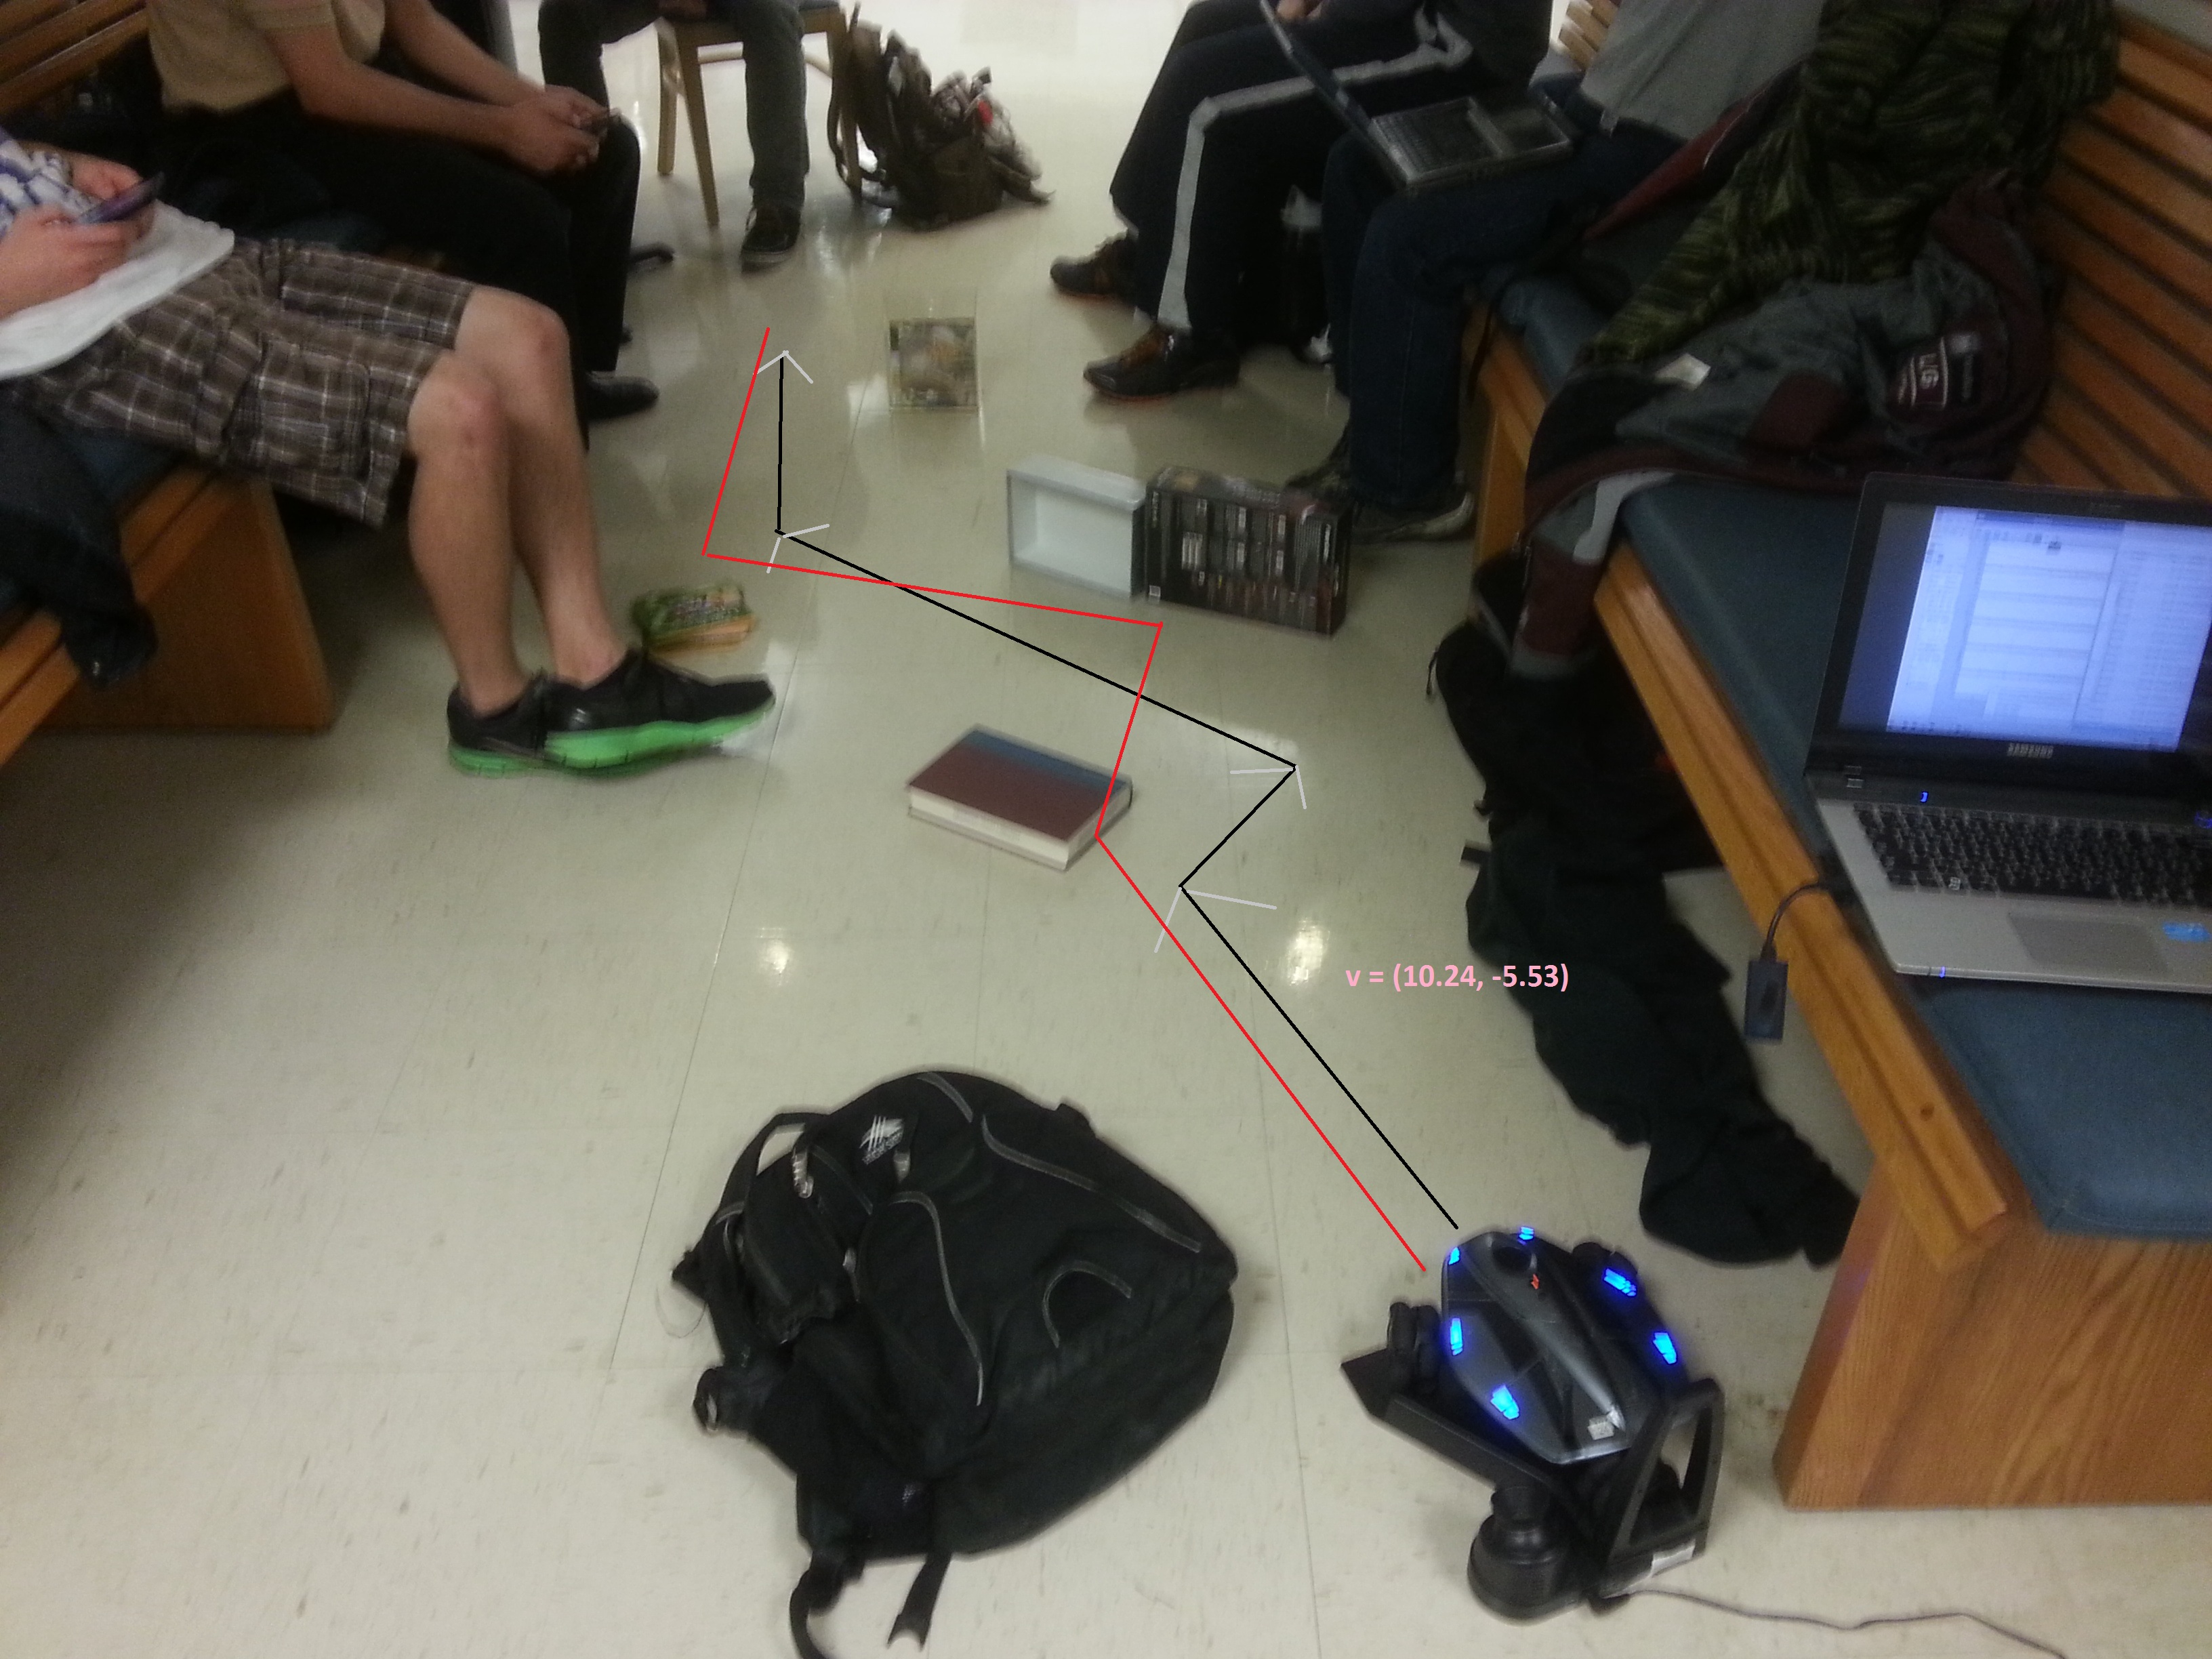
\includegraphics[width=12.5cm]{estimated.jpg} \\*
}

\vspace{8mm}
\bf Section 2.3: Trajectory from Dead Odometry \rm
\vspace{4mm}

From above, we remember that:
$$ \dot{\xi} = 
J\left[\begin{array}{c}
\dot{\phi_r} \\
\dot{\phi_l} \\
\dot{\phi_b}
\end{array}\right] \\* 
$$

 Now I am to take all of the encoder values for the commands and transform them into velocities using the Jacobian. And then I'll integrate these interval velocities over the command. \\
The first command is simple, with $\Delta t \approx 0.305$
$$
\dot{\xi}^1 = J(8, 8, 0)^T
$$

so for the first velocity, we get......
$$
\dot{\xi}^1 = (0.0352, -0.7064, 0.9368)^T
$$

woah... let's hope this doesn't continue, as this isn't making much sense. If it does, either I screwed up, or using a Jacobian is a bad way to estimate trajectories.

$$
\dot{\xi}^2 = J(12, 12, 0)^T
$$

$$
\dot{\xi}^2 = (0.0528, -1.0596, 1.4052)^T
$$

agh... not promising. But, still, we continue.


$$
\dot{\xi}^3 = J(30, 31, 0)^T
$$

$$
\dot{\xi}^3 = (-0.3679, -3.28, 0)^T
$$

Nope. The system is screwed.

$$
\dot{\xi}^4 = J(15, 15, 0)^T
$$

$$
\dot{\xi}^4 = (0.066, -1.3245, 1.7565)^T
$$

$$
\dot{\xi}^5 = J(10, 10, 0)^T
$$

$$
\dot{\xi}^5 = (0.044, -0.883, 1.171)^T
$$
Ok, this is really making me sad.

$$
\dot{\xi}^6 = J(12, 10, 0)^T
$$

$$
\dot{\xi}^6 = (1.0526, 0.2088, -0.2756)^T
$$

Finally! A reasonable-looking twist! Oh wait. It's the last one. \\

Well, I think I can say that this was an unadulterated failure.

I'll integrate these values to get a pose change, just for kicks. But, it's not going to be reasonable.
$$
\vec{x} = 0.309 * \dot{\xi}^1 + 0.341 * \dot{\xi}^2 + 0.301 * \dot{\xi}^3 + 0.301 * \dot{\xi}^4 + 0.27 * \dot{\xi}^5 + 0.38 * \dot{\xi}^6
$$
Therefore....
$$
\vec{x} = (0.3499, -2.1246, 1.5088)^T
$$

The path is visualized in Green. Profoundly bad. I'm not even going to continue with this. Look forwards to damage control on my Wordpress blog very soon!

{
\centering
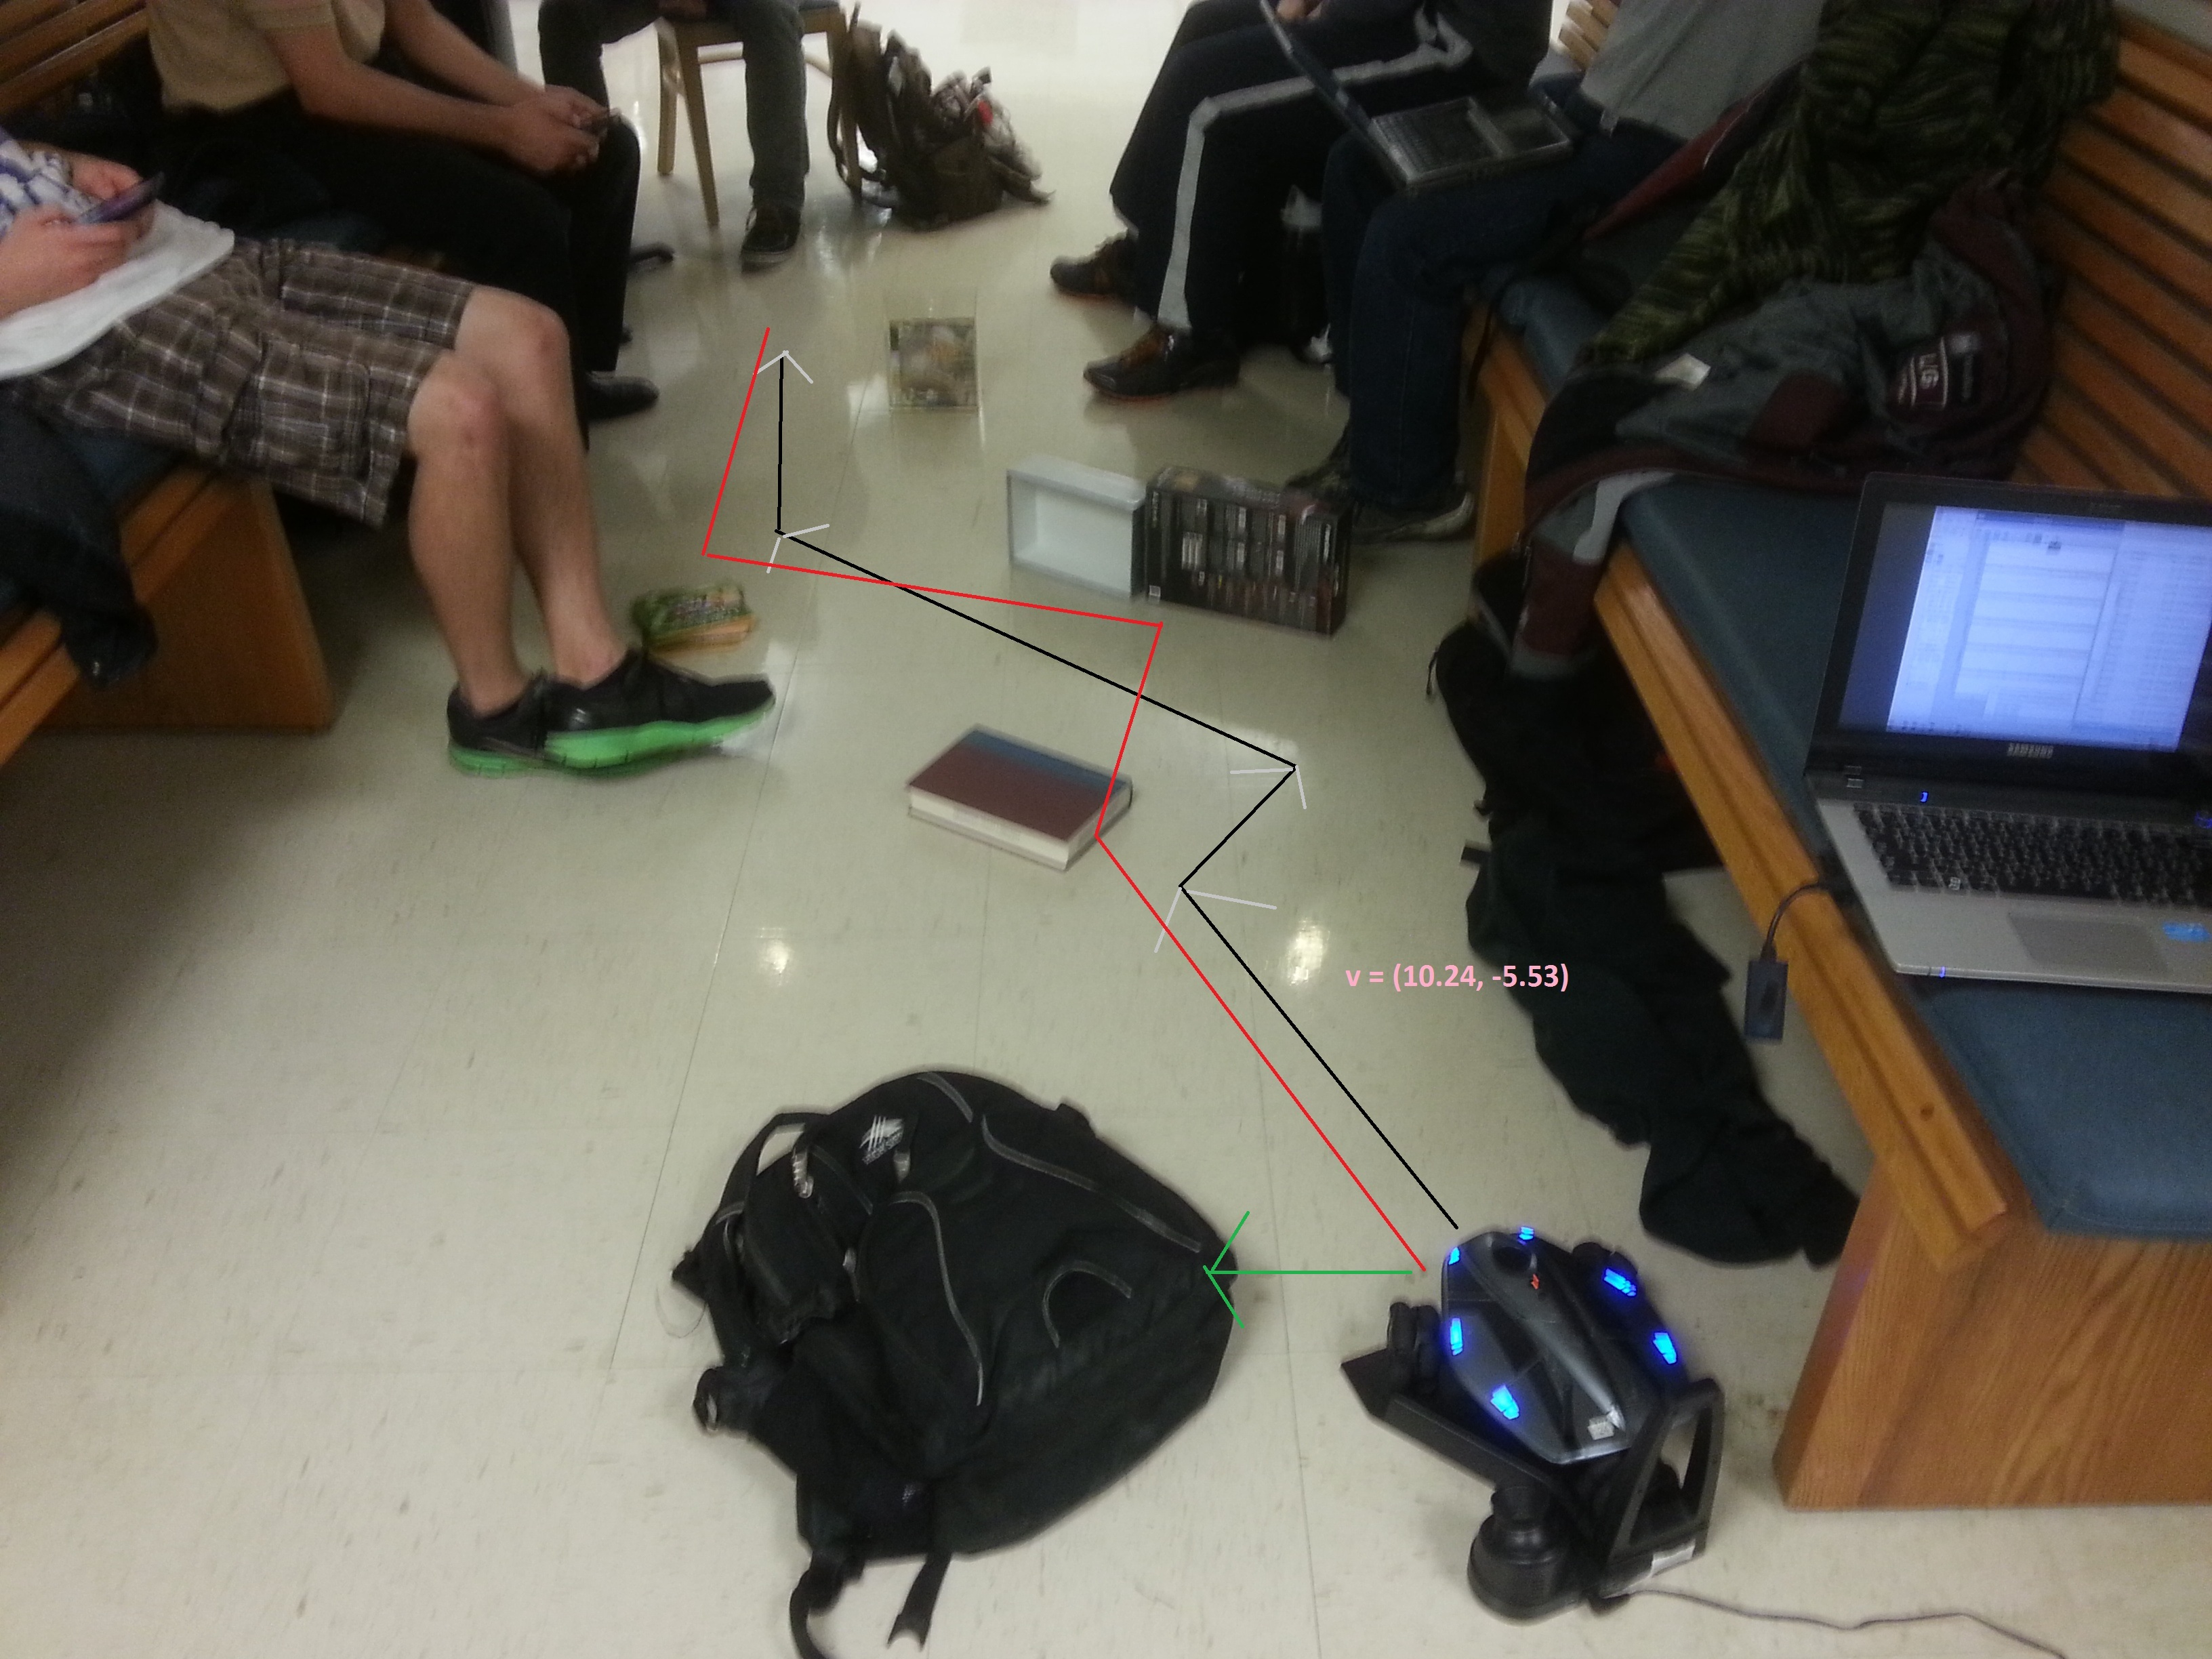
\includegraphics[width=9.5cm]{odometry.jpg} \\*
}
\end{document}



